% Options for packages loaded elsewhere
\PassOptionsToPackage{unicode}{hyperref}
\PassOptionsToPackage{hyphens}{url}
\documentclass[
]{article}
\usepackage{xcolor}
\usepackage{amsmath,amssymb}
\setcounter{secnumdepth}{-\maxdimen} % remove section numbering
\usepackage{iftex}
\ifPDFTeX
  \usepackage[T1]{fontenc}
  \usepackage[utf8]{inputenc}
  \usepackage{textcomp} % provide euro and other symbols
\else % if luatex or xetex
  \usepackage{unicode-math} % this also loads fontspec
  \defaultfontfeatures{Scale=MatchLowercase}
  \defaultfontfeatures[\rmfamily]{Ligatures=TeX,Scale=1}
\fi
\usepackage{lmodern}
\ifPDFTeX\else
  % xetex/luatex font selection
\fi
% Use upquote if available, for straight quotes in verbatim environments
\IfFileExists{upquote.sty}{\usepackage{upquote}}{}
\IfFileExists{microtype.sty}{% use microtype if available
  \usepackage[]{microtype}
  \UseMicrotypeSet[protrusion]{basicmath} % disable protrusion for tt fonts
}{}
\makeatletter
\@ifundefined{KOMAClassName}{% if non-KOMA class
  \IfFileExists{parskip.sty}{%
    \usepackage{parskip}
  }{% else
    \setlength{\parindent}{0pt}
    \setlength{\parskip}{6pt plus 2pt minus 1pt}}
}{% if KOMA class
  \KOMAoptions{parskip=half}}
\makeatother
\usepackage{graphicx}
\makeatletter
\newsavebox\pandoc@box
\newcommand*\pandocbounded[1]{% scales image to fit in text height/width
  \sbox\pandoc@box{#1}%
  \Gscale@div\@tempa{\textheight}{\dimexpr\ht\pandoc@box+\dp\pandoc@box\relax}%
  \Gscale@div\@tempb{\linewidth}{\wd\pandoc@box}%
  \ifdim\@tempb\p@<\@tempa\p@\let\@tempa\@tempb\fi% select the smaller of both
  \ifdim\@tempa\p@<\p@\scalebox{\@tempa}{\usebox\pandoc@box}%
  \else\usebox{\pandoc@box}%
  \fi%
}
% Set default figure placement to htbp
\def\fps@figure{htbp}
\makeatother
\setlength{\emergencystretch}{3em} % prevent overfull lines
\providecommand{\tightlist}{%
  \setlength{\itemsep}{0pt}\setlength{\parskip}{0pt}}
\usepackage{bookmark}
\IfFileExists{xurl.sty}{\usepackage{xurl}}{} % add URL line breaks if available
\urlstyle{same}
\hypersetup{
  hidelinks,
  pdfcreator={LaTeX via pandoc}}

\author{}
\date{}

\begin{document}

\section{Multirate Audio Equalizer}\label{multirate-audio-equalizer}

\subsection{48 kHz -\textgreater{} 44.1 kHz}\label{khz---44.1-khz}

\textbf{Please sketch the cascaded system of an upsampler by L followed
by a down-sampler by D. Is there any way to simplify this system and use
one low-pass filter instead of two?}
\pandocbounded{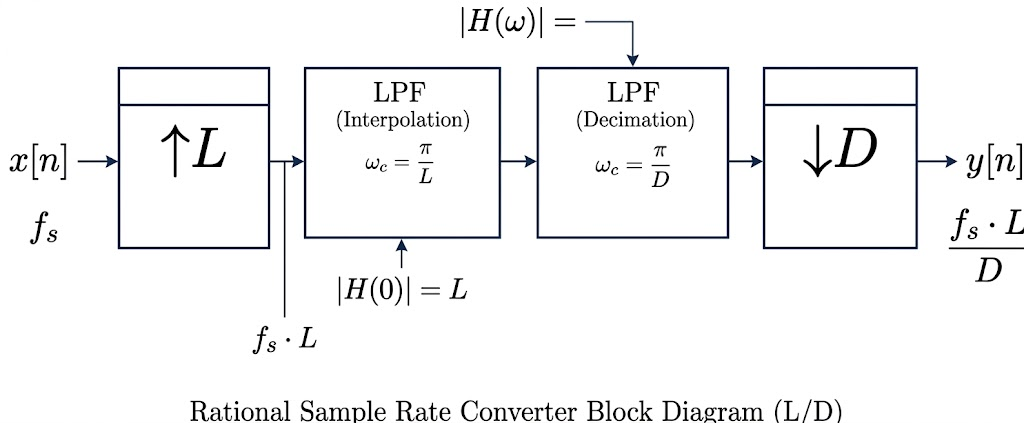
\includegraphics[keepaspectratio]{image.png}}

We can simplify the two LPFs since they are LTI (Linear Time Invariant,
we know this since H is defined) so they both operate at frequency fs*L.
To satisfy cutoff frequency, we use the minimum of wc/L and wc/D

\textbf{Please find the smallest integer values L and D that, when we
upsample by L and downsample by D, we convert 48 kHz to 44.1 kHz. (such
that L/D = 44100/48000). What sampling rate does the
anti-aliasing/anti-imaging filter process data at? If we use a FIR
filter with N taps, how many multiplications does this require per
second?}

L/D = 44100/48000 simplifies to 147/160. Since we know f = L\emph{fs,
and we know fs = 48kHz, f = 7.056 MHz, our filter's sampling rate. With
N taps, we multiply by FSR to get 7.056E(6) } N taps per second

\textbf{What passband gain do we need from our filter? What cutoff
frequency (in both hertz and in radians per sample)?}

Our passband gain is the product of our two individual gains: H\_aa *
H\_ai = H\_total -\textgreater{} L * 1 = L, which we know is 147.

w\_c = min(pi/160, pi/147) -\textgreater{} pi/160 In Hz -\textgreater{}
(pi/160) * f\_sr / 2pi -\textgreater{} fsr / 320 -\textgreater{} 22.05
kHz

\textbf{Is this h{[}n{]} finite-duration? Is it causal? Do you see any
issues implementing this with a computer?} For n\textless0, this
function is not non-zero, so it is not causal. It is not finite since as
$n \to \infty$, it does not permanently stay at 0 (rather it decays at
1/n, oscillating around it). Since it is not causal, and inifinite, we
cannot store this function in memory. Since it's not causal, we cannot
normally implement a live/real-time version.

\pandocbounded{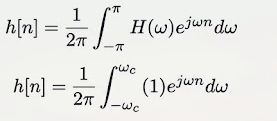
\includegraphics[keepaspectratio]{image-1.png}}

Using the following sin identity:

\pandocbounded{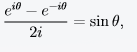
\includegraphics[keepaspectratio]{image-2.png}}
\pandocbounded{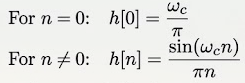
\includegraphics[keepaspectratio]{image-3.png}}

\textbf{Please take the (closed-form, analytical) h{[}n{]} you computed
in 3.1 and compute its values (in Python or MATLAB) over the range -M
\textless= n \textless= M, setting M = 10. Plot the DTFT of this
function. How does it differ from what you'd expect from an ideal
low-pass filter? Examine the DTFT for M = 100, M = 1000, and M = 10000.
What effect does increasing M appear to have? What differences still
exist between the M = 10000 case and the ideal low-pass filter?}

\pandocbounded{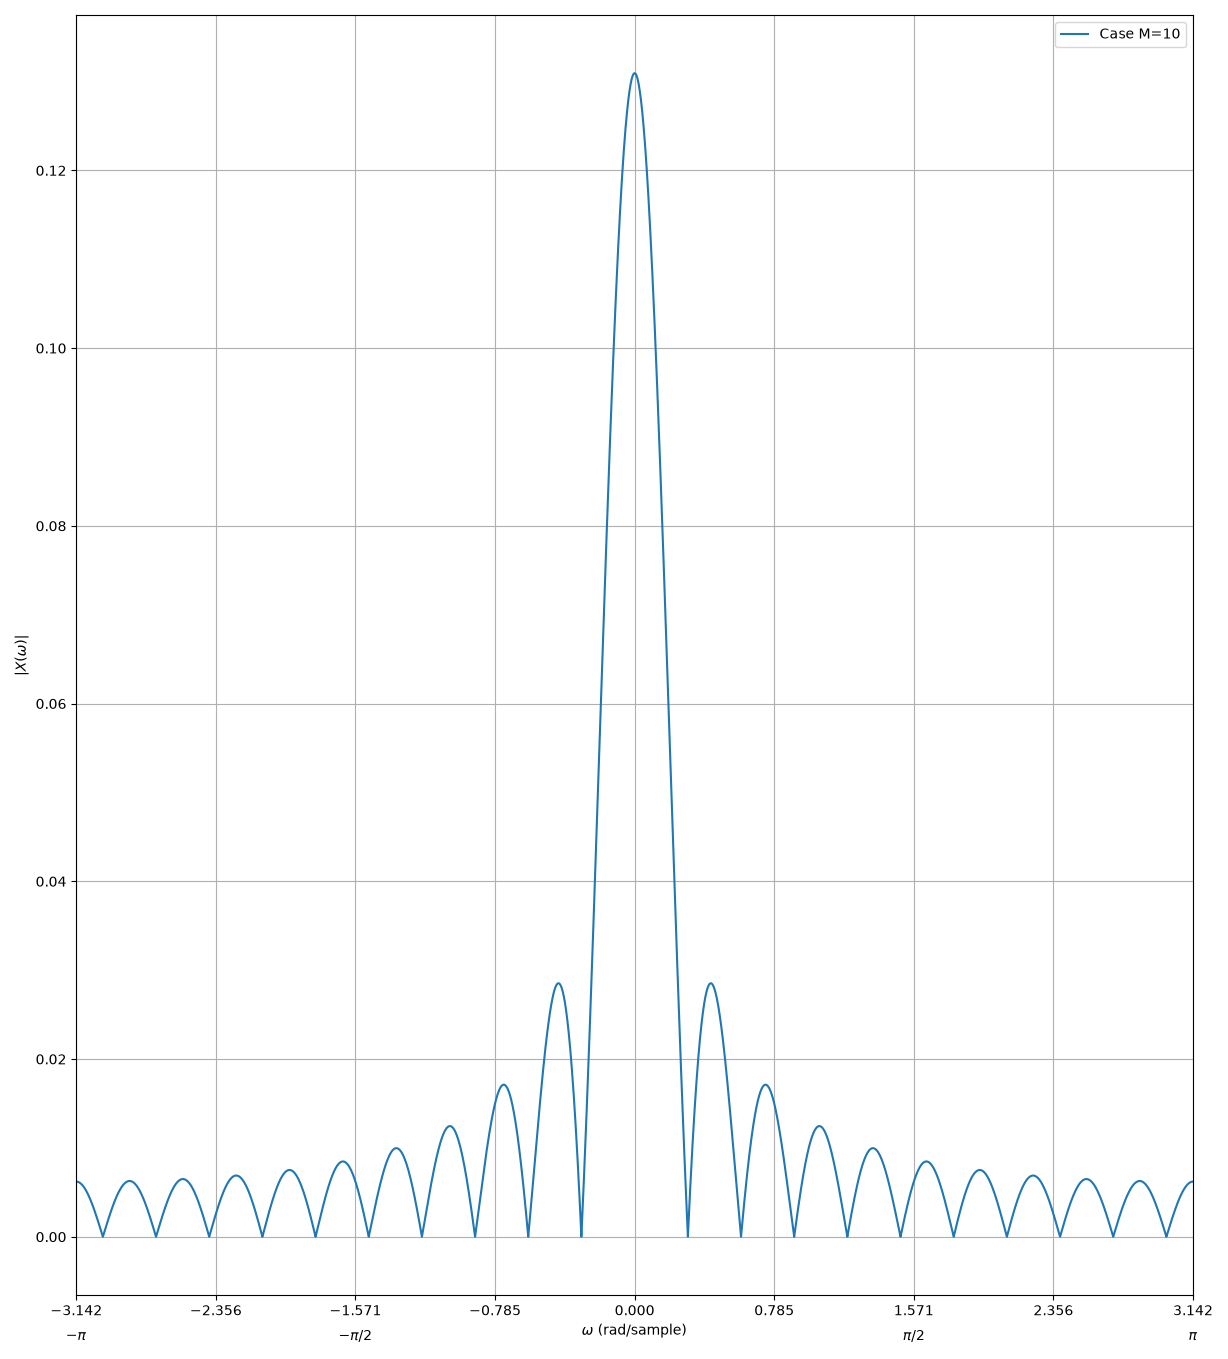
\includegraphics[keepaspectratio]{m10.png}} M = 10 case
\pandocbounded{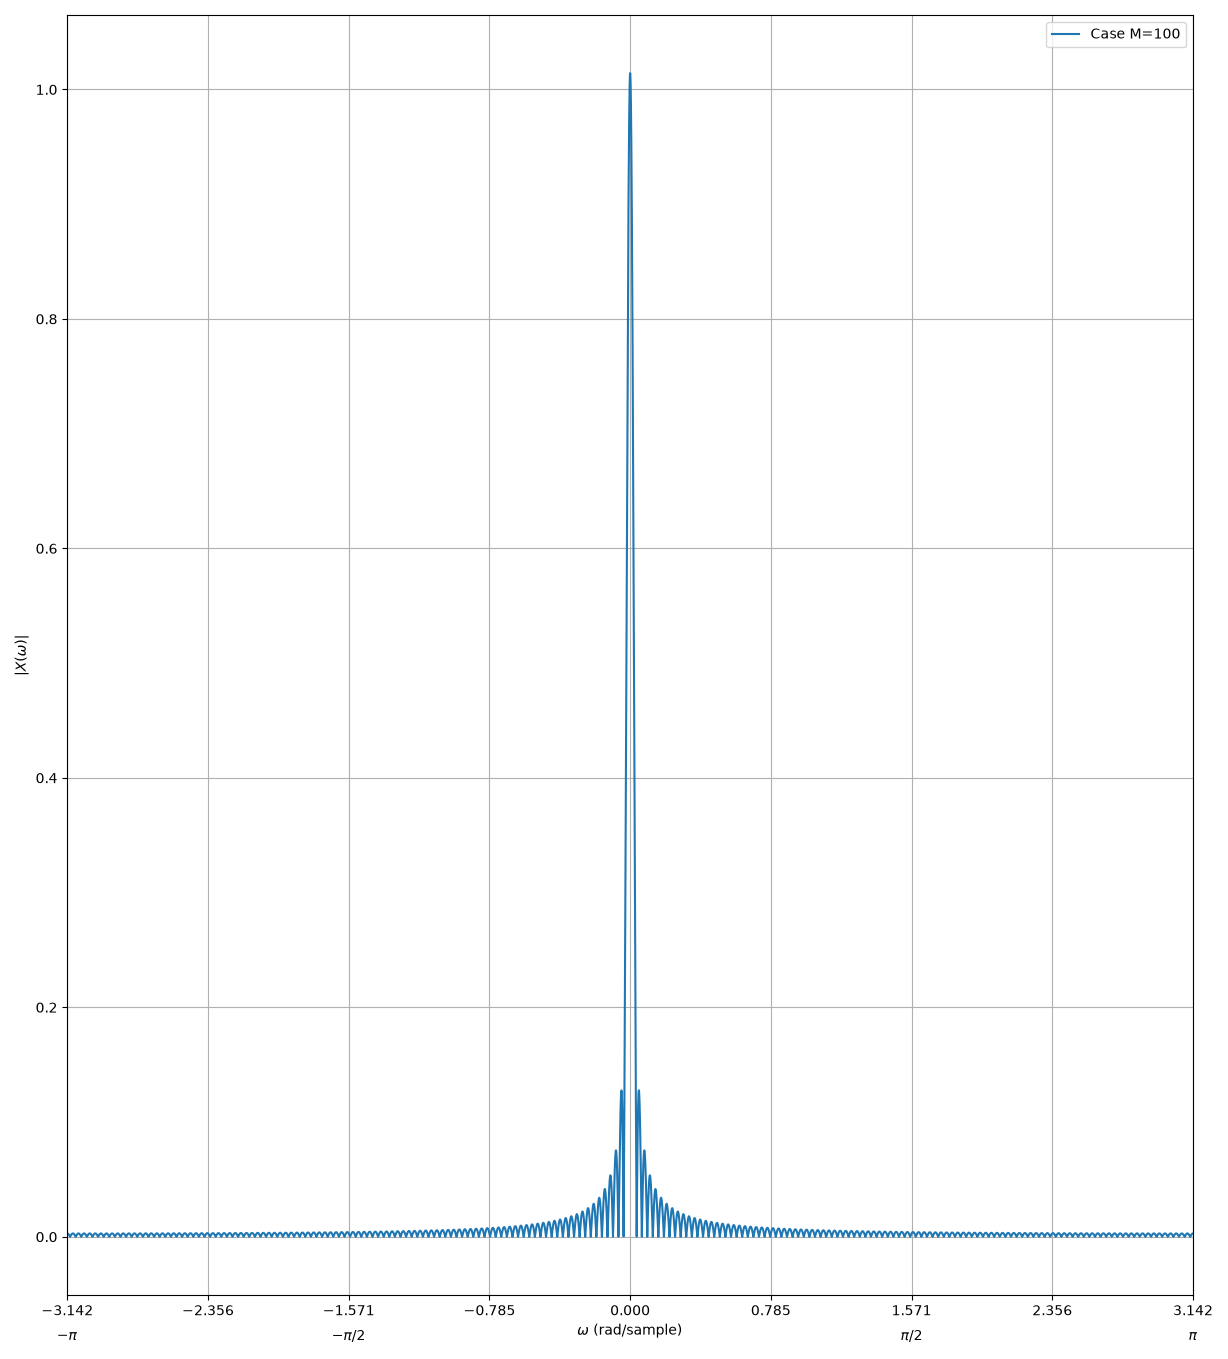
\includegraphics[keepaspectratio]{m100.png}} M = 100 case

\pandocbounded{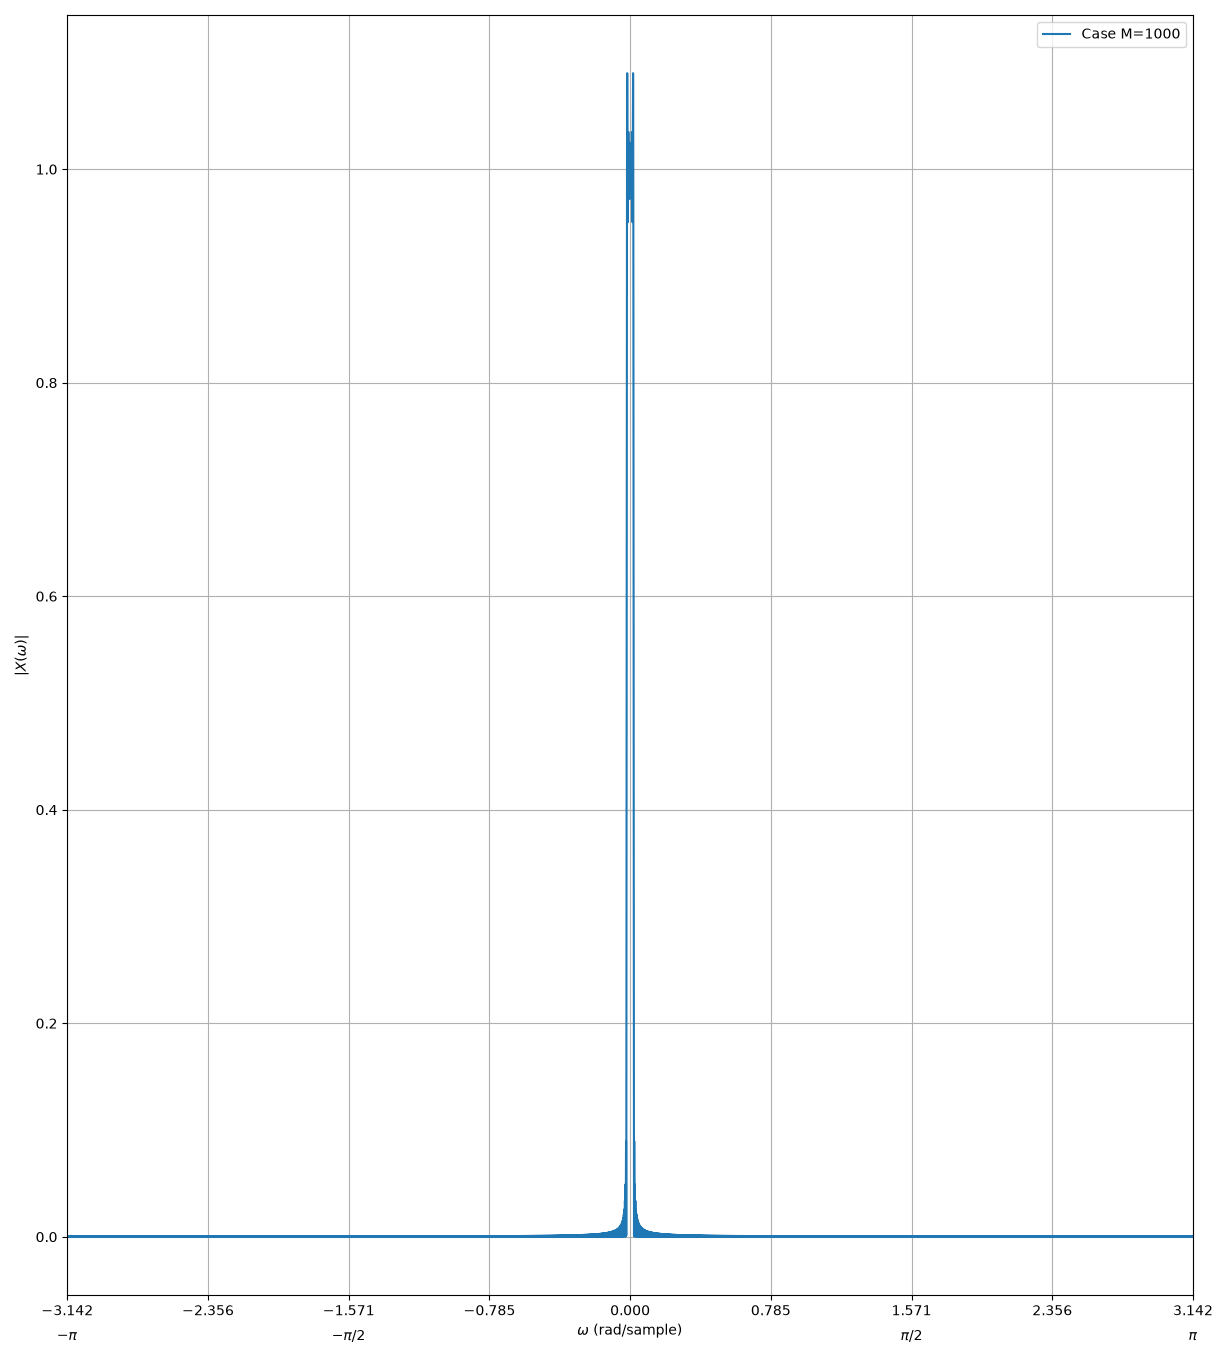
\includegraphics[keepaspectratio]{m1000.png}} M = 1000
case

\pandocbounded{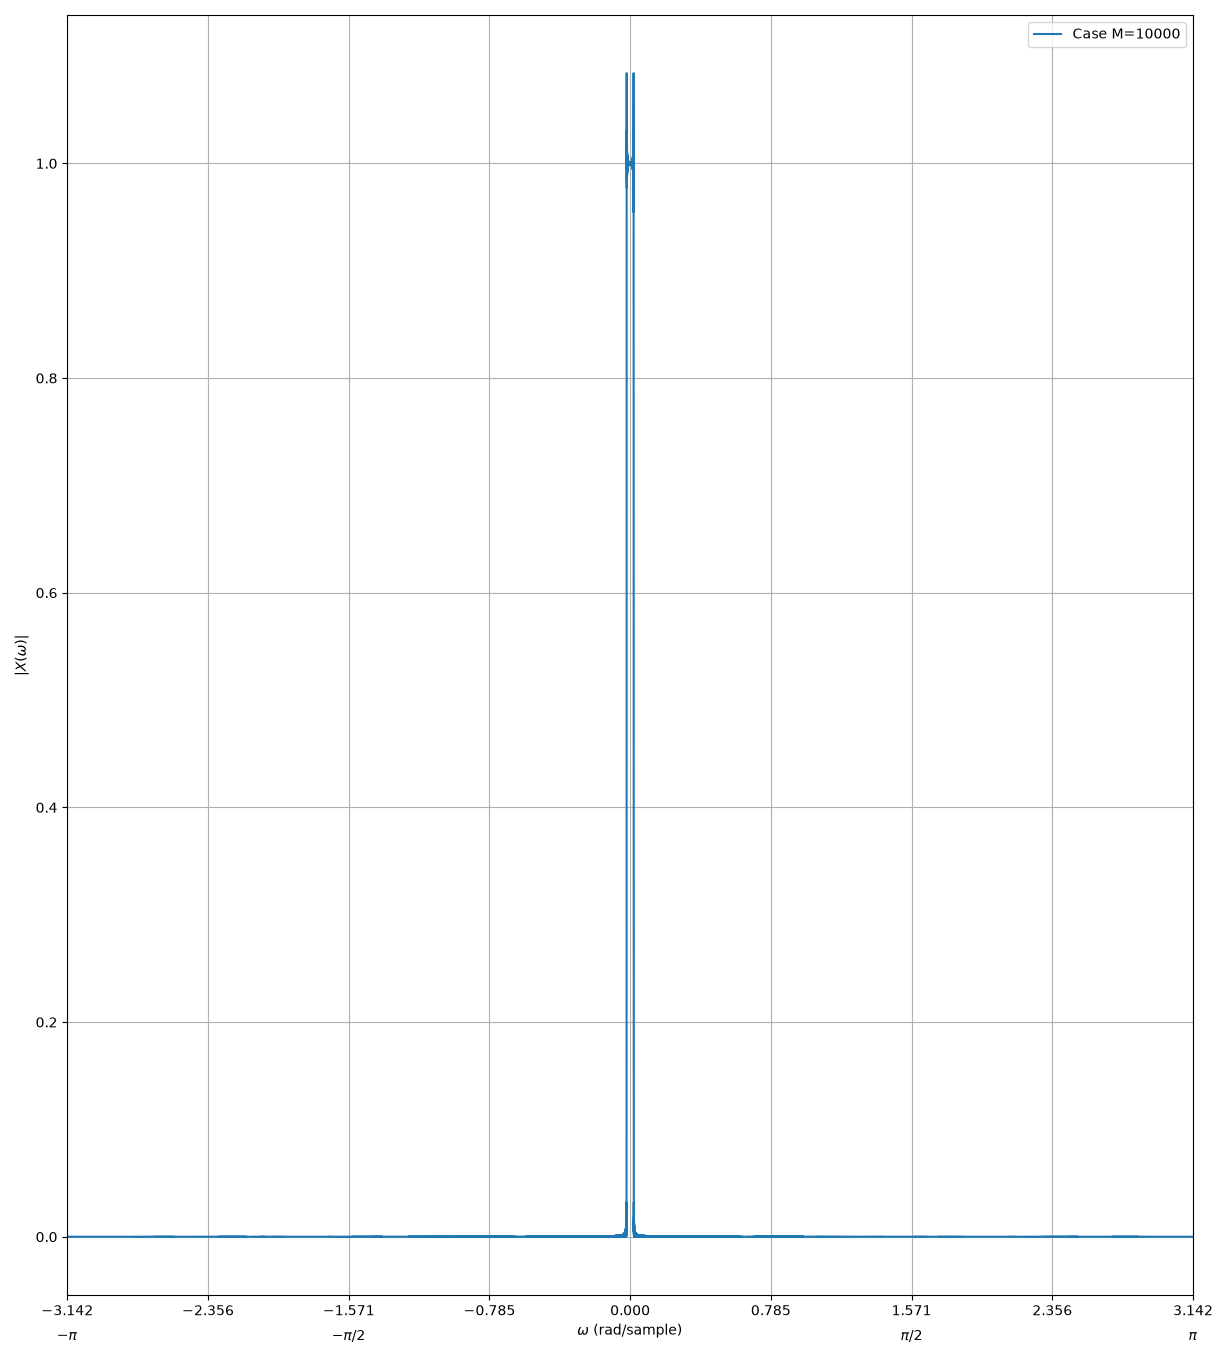
\includegraphics[keepaspectratio]{m10000.png}} M = 10000
case

For low values of M, the transition to the ideal gain (1) is very
apparent, and exhibits severe oscillation, creating obvious ripples. As
$M \to \infty$, the slope becomes much steeper and the ripples
disappear since they oscillate at higher frequency. But even for the
M=10000 case, there is overshoot over the ideal gain of 1

\textbf{What are two downsides to increasing the number of taps in an
FIR filter? For each, explain whether it matters to real-time filtering,
non-real-time (offline) filtering, or both.}

The two downsides are increased spacial and time complexity of the
program, and introduced latency.

Increased spacial and time complexity of the program applies to both
real-time and offline programs since you would have to wait longer for
computation in offline programs and for real-time, if you cannot compute
fast enough your program drops samples. Furthermore, for a large number
of taps, the program will quickly trigger an out-of-memory exception.

In terms of latency, the computer atrempts to make the program causal
through applying delays. A non-causal system looks like h{[}n{]} =
h{[}-n{]} for -M \textless= n \textless= M. To achieve causality, we
want h{[}n{]} = h{[}n-M{]} for 0 \textless= n \textless= 2M.

Then, n=0 corresponds to h{[}-M{]}, while N = 2M corresponds to h{[}M{]}
so we achieve our same range.

Since the time per sample is (1/fs), and number of samples = M, our
delay = M * 1/fs = M/fs. For a high M, say 10,000 and a sample rate of
48kHz, we see that delay = 0.2s per sample, incredibly high for a song.

For offline programs, this latency wouldn't really matter since the
computer will just wait to process it, increasing computation time but
achieving the same result. For a real-time program, we will immediately
notice the delay and lost parts of the song.

\end{document}
